% ---------------------------------------------------------------------
%  §4. Resultados
% ---------------------------------------------------------------------
\section{Resultados}

% =====================================================================
\subsection{Nivel de desarrollo del país}

Los estudiantes de \textbf{países en desarrollo} muestran resultados menos favorables en los cuatro
indicadores (Tabla~\ref{tab:desarrollo}): usan más las redes (5,25 horas diarias contra 4,83), duermen
menos (6,45 horas contra 6,97), tienen un puntaje de salud mental más bajo (5,94 contra 6,37) y declaran con
mayor frecuencia que las redes afectan su rendimiento académico (74\,\% contra 56\,\%). La diferencia en el
descanso alcanza a toda la distribución (Figura~\ref{fig:sueno_desarrollo}): la mediana es de 6,3 horas
por noche contra 7,1, y la mitad central de cada grupo se ubica más abajo en los países en desarrollo
(entre 5,7 y 7,2 horas) que en los desarrollados (entre 6,1 y 7,8 horas), con una dispersión parecida.

\begin{table}[H]
\centering
\small
\caption{Indicadores según el nivel de desarrollo del país (media y mediana).}
\label{tab:desarrollo}
\begin{tabular}{l cc cc cc c}
\toprule
& \multicolumn{2}{c}{\textbf{Uso diario (h)}} & \multicolumn{2}{c}{\textbf{Sueño (h)}}
& \multicolumn{2}{c}{\textbf{Salud mental}} & \textbf{Afecta rend.} \\
\cmidrule(lr){2-3}\cmidrule(lr){4-5}\cmidrule(lr){6-7}\cmidrule(lr){8-8}
\textbf{Nivel de desarrollo} & Media & Mediana & Media & Mediana & Media & Mediana & \% Sí \\
\midrule
Desarrollado ($n=1.103$)  & 4,83 & 4,6 & 6,97 & 7,1 & 6,37 & 6,3 & 56,48 \\
En desarrollo ($n=638$)   & 5,25 & 5,2 & 6,45 & 6,3 & 5,94 & 6,0 & 74,45 \\
\bottomrule
\end{tabular}
\end{table}

% =====================================================================
\subsection{Uso de redes, sueño y rendimiento académico}

Se observa una clara relación negativa entre el uso de redes y el descanso (Figura~\ref{fig:uso_sueno}):
la correlación es de $\mathbf{-0{,}79}$ y, según la recta de tendencia, cada hora adicional de uso diario se
asocia en promedio con unas \textbf{0,65 horas menos de sueño}.

\begin{figure}[H]
\centering
\begin{subfigure}[t]{0.46\linewidth}
  \centering
  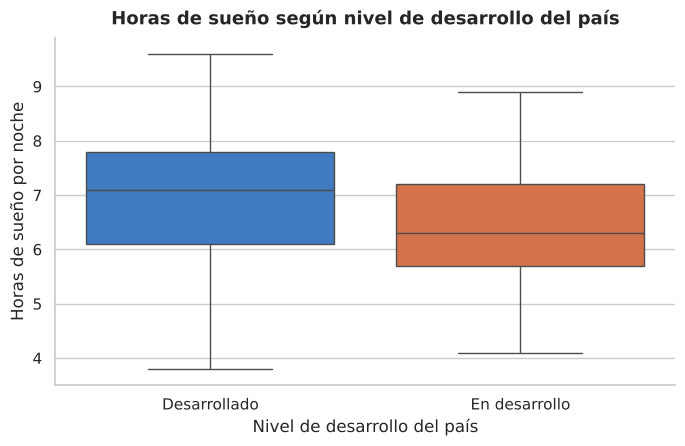
\includegraphics[width=\linewidth]{fig01_sueno_desarrollo.png}
  \caption{Según nivel de desarrollo del país.}
  \label{fig:sueno_desarrollo}
\end{subfigure}\hspace{0.03\linewidth}
\begin{subfigure}[t]{0.38\linewidth}
  \centering
  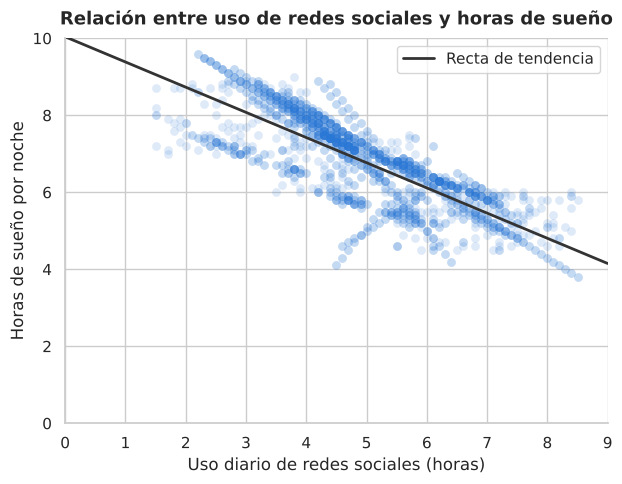
\includegraphics[width=\linewidth]{fig02_uso_sueno.png}
  \caption{Según uso diario de redes, con recta de tendencia.}
  \label{fig:uso_sueno}
\end{subfigure}
\caption{Horas de sueño por noche de los estudiantes.}
\label{fig:sueno}
\end{figure}

El 63\,\% de los estudiantes (1.100 de 1.743) declara que las redes afectan su rendimiento académico, y
quienes se sienten perjudicados se concentran en la zona de más horas de uso y menos horas de sueño
(Figura~\ref{fig:uso_sueno_impacto}). Este grupo usa las redes 1,7 horas más por día y duerme 1,4 horas
menos que el resto (Tabla~\ref{tab:academico}); las medianas son casi iguales a las medias, por lo que la
diferencia no se debe a unos pocos casos extremos. La brecha más marcada aparece en el descanso: \textbf{el
77\,\% de los que se sienten afectados duerme menos de 7 horas}, el mínimo recomendado para adultos
\cite{watson}, contra el 13\,\% del otro grupo.

\begin{figure}[H]
\centering
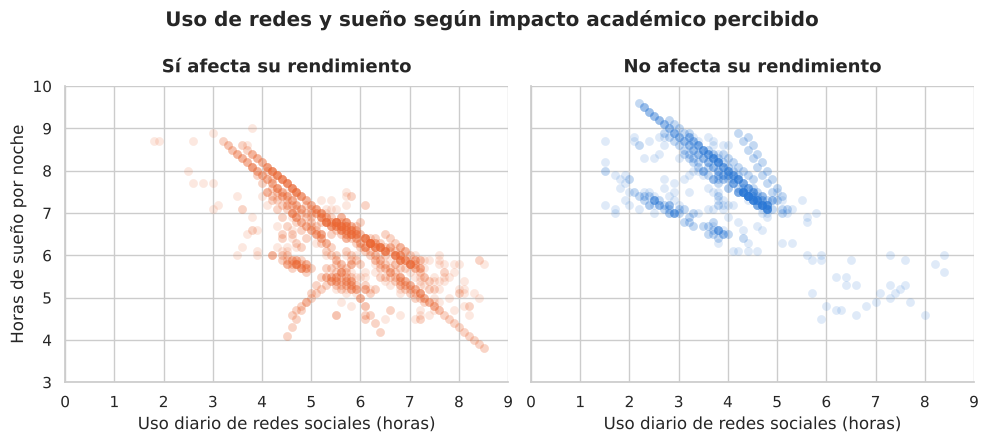
\includegraphics[width=0.60\linewidth]{fig03_uso_sueno_impacto.png}
\caption{Uso de redes y sueño según el impacto académico percibido.}
\label{fig:uso_sueno_impacto}
\end{figure}

\begin{table}[H]
\centering
\small
\caption{Uso y sueño según el impacto académico percibido.}
\label{tab:academico}
\begin{tabular}{l c cc cc c}
\toprule
\textbf{¿Las redes afectan} & & \multicolumn{2}{c}{\textbf{Uso diario (h)}} & \multicolumn{2}{c}{\textbf{Sueño (h)}} & \textbf{Duerme} \\
\cmidrule(lr){3-4}\cmidrule(lr){5-6}
\textbf{su rendimiento?} & \textbf{Estudiantes} & Media & Mediana & Media & Mediana & \textbf{< 7 h (\%)} \\
\midrule
No & 643   & 3,88 & 3,9 & 7,65 & 7,6 & 13,06 \\
Sí & 1.100 & 5,62 & 5,6 & 6,27 & 6,2 & 76,64 \\
\bottomrule
\end{tabular}
\end{table}

% =====================================================================
\subsection{Plataformas y brecha de género}

\textbf{Diferencias entre plataformas.} Sobre los 1.038 estudiantes sin duplicados se observan grandes
diferencias según la red más usada (Tabla~\ref{tab:plataforma}). \textbf{WhatsApp} muestra los resultados
más preocupantes: más horas de uso (6,5 h), menos sueño (5,9 h), la peor salud mental (5,54) y el
100\,\% de sus usuarios declara que las redes afectan su rendimiento. Le siguen \textbf{TikTok} (5,77) y
\textbf{Snapchat} (5,81). En el otro extremo, \emph{Otras} (6,84), \textbf{LinkedIn} (6,77),
\textbf{Twitter} (6,57) y \textbf{Facebook} (6,51) combinan mejor salud mental, más sueño y menor
afectación académica; Instagram, la más usada, queda en una posición intermedia (6,15).

\begin{table}[H]
\centering
\footnotesize
\setlength{\tabcolsep}{4pt}
\caption{Indicadores promedio según la plataforma más usada, ordenados de peor a mejor salud mental, y
salud mental promedio dentro de cada nivel de uso diario.}
\label{tab:plataforma}
\begin{tabular}{l ccccc ccc}
\toprule
& & & & & & \multicolumn{3}{c}{\textbf{Salud mental por nivel de uso}} \\
\cmidrule(lr){7-9}
\textbf{Plataforma} & \textbf{Uso (h)} & \textbf{Sueño (h)} & \textbf{Salud m.} & \textbf{Afecta} & \textbf{$n$}
& \textbf{Bajo ($\leq$4 h)} & \textbf{Medio (4--6 h)} & \textbf{Alto ($>$6 h)} \\
\midrule
WhatsApp  & 6,48 & 5,87 & 5,54 & 1,00 & 54  & --   & 5,82 & 5,41 \\
TikTok    & 5,38 & 6,32 & 5,77 & 0,85 & 196 & 7,11 & 5,89 & 4,87 \\
Snapchat  & 5,54 & 6,01 & 5,81 & 0,77 & 60  & 7,43 & 5,87 & 4,99 \\
Instagram & 4,88 & 6,96 & 6,15 & 0,65 & 301 & 7,42 & 6,04 & 4,72 \\
YouTube   & 4,91 & 6,51 & 6,34 & 0,52 & 65  & 7,46 & 5,98 & 5,09 \\
Facebook  & 4,83 & 7,08 & 6,51 & 0,41 & 172 & 7,64 & 6,63 & 4,86 \\
Twitter   & 4,89 & 6,67 & 6,57 & 0,51 & 73  & 7,49 & 6,72 & 5,05 \\
LinkedIn  & 4,23 & 6,82 & 6,77 & 0,33 & 66  & 7,82 & 6,17 & 4,64 \\
Otras     & 4,34 & 7,61 & 6,84 & 0,39 & 51  & 7,67 & 6,39 & --   \\
\midrule
\multicolumn{6}{l}{\textbf{Promedio de cada nivel de uso (todas las plataformas)}} & \textbf{7,51} & \textbf{6,16} & \textbf{4,93} \\
\bottomrule
\end{tabular}

\smallskip
{\footnotesize\textit{Nota:} “Afecta” es la proporción de estudiantes que declara que las redes afectan su
rendimiento (0,33 equivale al 33\,\%); $n$ es la cantidad de estudiantes; “--” indica que no hay
estudiantes en esa combinación.}
\end{table}

En la Figura~\ref{fig:uso_salud_plataforma} cada punto es una plataforma y los puntos bajan de izquierda
a derecha: \textbf{cuantas más horas de uso promedio tiene una plataforma, menor es la salud mental promedio
de sus usuarios}. WhatsApp acumula más horas y el peor puntaje; LinkedIn y \emph{Otras}, el menor uso
(alrededor de 4,3 h) y los mejores puntajes. Una hipótesis es que las plataformas de uso constante y alta
frecuencia se asocian con más horas de pantalla, y las de uso puntual con menos.

\begin{figure}[H]
\centering
\begin{subfigure}[t]{0.46\linewidth}
  \centering
  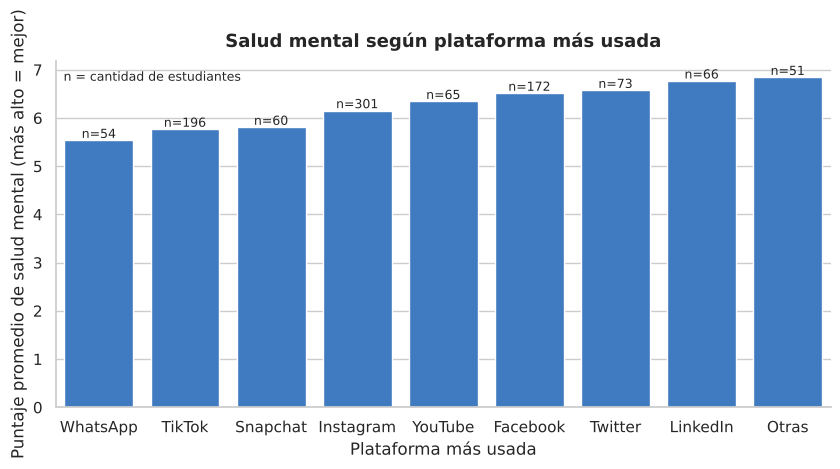
\includegraphics[width=\linewidth]{fig05_salud_plataforma.png}
  \caption{Salud mental promedio por plataforma.}
  \label{fig:salud_plataforma}
\end{subfigure}\hspace{0.03\linewidth}
\begin{subfigure}[t]{0.42\linewidth}
  \centering
  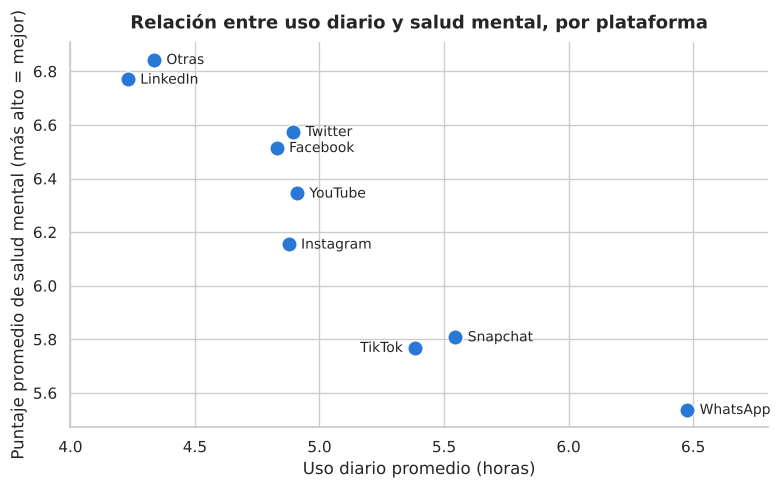
\includegraphics[width=\linewidth]{fig06_uso_salud_plataforma.png}
  \caption{Uso diario y salud mental promedio, por plataforma.}
  \label{fig:uso_salud_plataforma}
\end{subfigure}
\caption{Salud mental según la plataforma más usada.}
\label{fig:plataformas}
\end{figure}

\textbf{¿Es la plataforma o son las horas?} A nivel general, cuantas más horas se usan las redes, peor es
la salud mental (correlación de $-0{,}82$): el puntaje baja de 7,51 en el uso bajo a 6,16 en el medio y a
4,93 en el alto. Al comparar estudiantes con una cantidad de horas parecida (columnas derechas de la
Tabla~\ref{tab:plataforma}), las diferencias entre plataformas se achican de 1,3 puntos a entre 0,7 y 0,9:
\textbf{gran parte de la diferencia entre plataformas se debe a las horas de uso y no a la plataforma en
sí}. Aun así, en los niveles bajo y medio la diferencia no desaparece: entre quienes usan las redes de 4 a 6
horas, TikTok (5,89) y Snapchat (5,87) siguen por debajo de Facebook (6,63) y Twitter (6,72). Con un uso muy
intensivo, en cambio, el orden se mezcla: Facebook (4,86) queda a la par de TikTok (4,87), WhatsApp pasa a
tener el mejor promedio (5,41) y LinkedIn el peor (4,64). Las diferencias que persisten pueden deberse a la
plataforma o a que quienes la eligen sean distintos; con estos datos no es posible distinguirlo.

\begin{wrapfigure}{r}{0.42\linewidth}
\vspace{-1.2em}
\centering
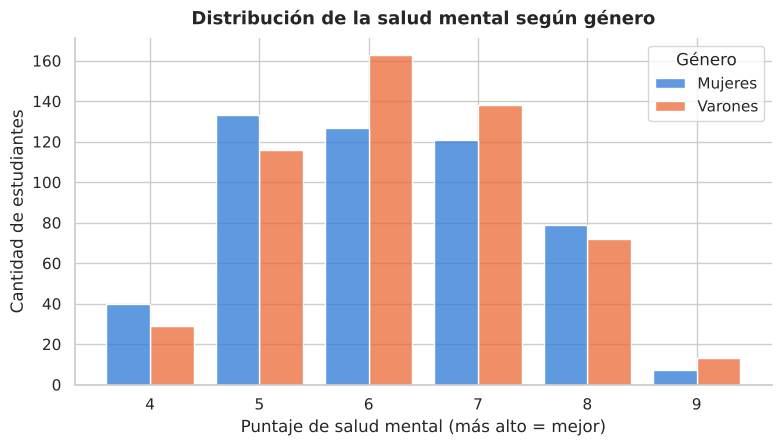
\includegraphics[width=\linewidth]{fig04_salud_genero.png}
\caption{Distribución del puntaje de salud mental según género.}
\label{fig:genero}
\vspace{-1em}
\end{wrapfigure}

\textbf{Brecha de género.} Las diferencias por género son muy chicas: mujeres y varones usan las redes
alrededor de 5 horas por día (5,08 contra 4,96), duermen cerca de 6,7 horas (6,68 contra 6,76) y la
afectación académica es casi idéntica (63\,\% contra 62\,\%). En salud mental los varones promedian 6,25 y
las mujeres 6,15, una diferencia de \textbf{0,10 puntos} con la misma mediana (6,0); ambas distribuciones
van del mismo mínimo al mismo máximo y concentran la mayoría de los casos entre 5 y 7
(Figura~\ref{fig:genero}). Dentro de cada plataforma las brechas también son chicas (0,42 puntos o menos,
la mayor en Snapchat, con pocos estudiantes) y \textbf{cambian de signo}: en Instagram, Twitter y
\emph{Otras} las mujeres tienen un puntaje levemente mayor, y en Snapchat, WhatsApp y Facebook, los
varones. La diferencia de género aparece, en cambio, en \emph{quién} usa cada red: Instagram es
mayoritariamente femenina (193 mujeres y 108 varones), mientras que Facebook (120 varones y 52 mujeres) y
WhatsApp (43 varones y 11 mujeres) son mayoritariamente masculinas. Por lo tanto, el género no explica que
unas plataformas se asocien con mejor o peor salud mental que otras.

% =====================================================================
\subsection{Relaciones sentimentales}

Entre los 705 estudiantes con estado sentimental informado, 384 están solteros, 289 en pareja y 32 en
una situación complicada. La media y la mediana del uso diario son muy parecidas en los tres grupos, entre
4,7 y 4,9 horas por día (Figura~\ref{fig:uso_estado}), por lo que no se observa una diferencia en la
cantidad de uso según la situación sentimental. La diferencia aparece en \emph{qué} plataforma se usa.
Como varias redes tienen pocas observaciones con este dato, la comparación se concentra en las tres más
usadas: Instagram (249), TikTok (154) y Facebook (123). La proporción de solteros es mayor en
\textbf{TikTok (65,6\,\%)} y en \textbf{Instagram (58,2\,\%)}, mientras que en \textbf{Facebook} la mayoría
está en pareja (57,7\,\%) (Figura~\ref{fig:estado_top3}). Las situaciones complicadas son algo más
frecuentes en TikTok (5,2\,\%) e Instagram (4,0\,\%) que en Facebook (0,8\,\%), aunque se trata de muy pocos
estudiantes (8, 10 y 1), por lo que esa diferencia es poco confiable.

\begin{figure}[H]
\centering
\begin{subfigure}[t]{0.46\linewidth}
  \centering
  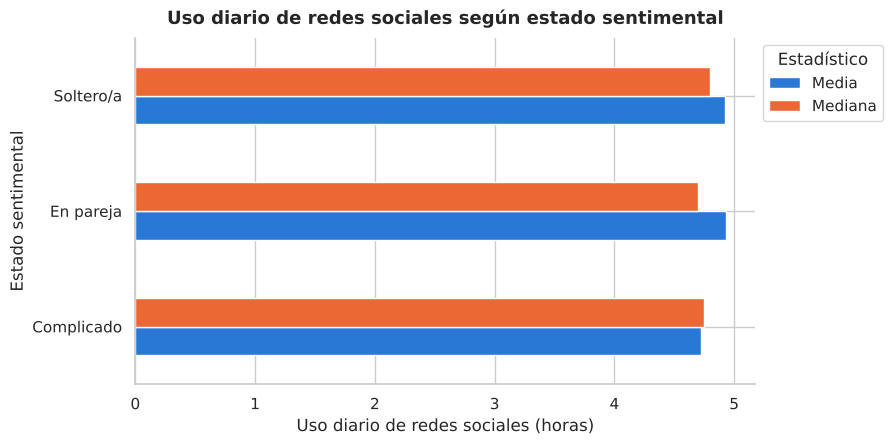
\includegraphics[width=\linewidth]{fig07_uso_estado_sentimental.png}
  \caption{Uso diario (media y mediana) según estado sentimental.}
  \label{fig:uso_estado}
\end{subfigure}\hspace{0.03\linewidth}
\begin{subfigure}[t]{0.44\linewidth}
  \centering
  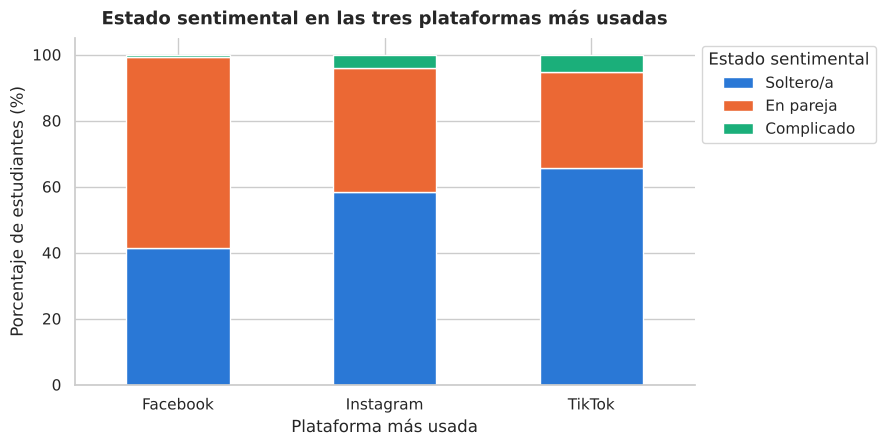
\includegraphics[width=\linewidth]{fig08_estado_top3.png}
  \caption{Estado sentimental en las tres plataformas más usadas.}
  \label{fig:estado_top3}
\end{subfigure}
\caption{Uso de redes sociales y situación sentimental.}
\label{fig:sentimental}
\end{figure}
